\documentclass{article}
%------------------------- packages -------------------------%
\usepackage[vietnamese.licr]{babel}
\usepackage{listings}
\usepackage{tvietlistings}
\usepackage[T1]{fontenc}
\usepackage[utf8]{inputenc} % Đảm bảo sử dụng mã hóa UTF-8
\usepackage{float}
\usepackage[many]{tcolorbox}
\usepackage[unicode,hidelinks]{hyperref}    % for reference
\usepackage{geometry}   % for layout
\usepackage{amsmath}    % for math
\usepackage{xcolor}     % for color
% for figure
\usepackage{graphicx}
\usepackage{caption}    
% for code
\usepackage{minted}
\usepackage[normalem]{ulem}
% for table
\usepackage{xparse}
\usepackage{float}      
\usepackage{paracol}
\usepackage{array}
\usepackage{multirow}
% for header & footer 
\usepackage{fancyhdr}
\usepackage{lastpage}
\usepackage{CJKutf8}
\usepackage{xcolor}


%------------------------- set up -------------------------%
% figure
\graphicspath{{./Images/}}              % path to image
\captionsetup[figure]{labelfont={small,bf,it},textfont={small,it}}
% paragraph
\setlength{\parindent}{0pt}
\setlength{\parskip}{12pt}
\setlength{\parskip}{6pt}               % disables indentation
\renewcommand{\baselinestretch}{1.5}    % line spacing

% code
\def\code#1{\texttt{#1}}    % font
\usemintedstyle{vs}         % minted theme
\setminted{
    autogobble,             % remove all common leading whitespace
    baselinestretch=1.0,
    bgcolor=gray!5!white,
    breaklines,
    %linenos,               % enables line numbers
    fontsize=\footnotesize
}
% Table addrow Macro with dyanamic
% Define the new addrow command to accept a variable number of arguments
\NewDocumentCommand{\addrow}{>{\SplitList{;}}m}{%
  \processline#1\relax
}


% Define a custom style
\lstdefinestyle{myStyle}{
    frame=l,
    framesep=4.5mm,
    framexleftmargin=2.5mm,
    basicstyle=\ttfamily\footnotesize,
    captionpos=b,
    commentstyle=\color{comment},
    breakatwhitespace=false,         
    breaklines=true,                 
    keepspaces=true,                 
    numbers=left,       
    numbersep=5pt,                  
    showspaces=false,                
    showstringspaces=false,
    showtabs=false,                  
    tabsize=2,
    keywords={if, else, for, while, repeat, function, in, next, break, library, ifelse, select, return, print, mutate, hist, tapply, apply, sapply, boxplot, barplot, factor},
		% keywordstyle=\color{blue}\bfseries,
        keywordstyle=\color{comment},
		ndkeywords={class, data.frame, numeric, matrix, character, list, c, seq},
		ndkeywordstyle=\color{black}\bfseries,
		identifierstyle=\color{black},
		sensitive=false,
		comment=[l]{\#},
}
% Helper macro to process each item
\newcommand{\processline}[1]{%
  \ifx\relax#1\relax % End of the list
    \\ \hline
  \else
    #1%
    \expandafter\processnext
  \fi
}

\newcommand{\processnext}[1]{%
  \ifx\relax#1\relax % End of the list
    \\ \hline
  \else
    & #1%
    \expandafter\processnext
  \fi
}

% Callout
\definecolor{main}{HTML}{5989cf}    % setting main color to be used
\definecolor{comment}{HTML}{606060}
\definecolor{sub}{HTML}{cde4ff}     % setting sub color to be used
\newtcolorbox{boxH}{
    % fontupper = \bf,
    boxrule = 1.5pt,
    colback = white, 
    colframe = black % frame color
}
% End
%------------------------- layout & margin -------------------------%
\geometry{
    a4paper,        % redundant if already in \documentclass
    left=20.32mm,
    right=20.32mm,
    top=25.40mm,
    bottom=25.40mm,
    heightrounded,  % better use it
}
\setlength{\parindent}{20pt}
%------------------------- header & footer -------------------------%
\renewcommand{\headrulewidth}{0.5pt}
\renewcommand{\footrulewidth}{0.5pt}
\setlength{\headheight}{24.5pt}
\pagestyle{fancy}

\fancyhead{}    % clear all header fields
\fancyhead[L]{
    \begin{tabular}{ll}
        \begin{picture}(10,10)
            \put(0,-7){
\includegraphics[width=8mm]{{Images/bachkhoa_logo.png}}}
        \end{picture}&
    	\begin{tabular}{l}
    	    {\ttfamily Trường Đại học Bách Khoa Tp. Hồ Chí Minh} \\
    	    {\ttfamily Khoa Khoa học và Kỹ thuật Máy tính} \\
    	\end{tabular} 	
    \end{tabular}
}

\fancyfoot{}    % clear all footer fields
\fancyfoot[L]{\footnotesize {\ttfamily Báo cáo bài tập lớn Xác Suất Thống Kê Kì 241}}
\fancyfoot[R]{\footnotesize {\ttfamily Trang {\thepage}/\pageref{LastPage}}}
% might change to \scriptsize

%------------------------- body -------------------------%
\begin{document}


% Use \lstset to make myStyle the global default
\lstset{style=myStyle}
%-------------------- cover --------------------%
\begin{titlepage}
\begin{center}
    \large ĐẠI HỌC QUỐC GIA THÀNH PHỐ HỒ CHÍ MINH \\
    TRƯỜNG ĐẠI HỌC BÁCH KHOA \\
    KHOA KHOA HỌC VÀ KỸ THUẬT MÁY TÍNH
\end{center}

\vspace{1.5cm}

\begin{figure}[!ht]
    \centering 
\includegraphics[width=3.5cm]{Images/bachkhoa_logo.png}
\end{figure}

\vspace{1.5cm}

\begin{table}[H]
    \centering
    \begin{tabular}{c}
    {\bf \Large XÁC SUẤT THỐNG KÊ (MT2013)} \\ \\
    \hline  \\
    \multicolumn{1}{l}{{\bf \large Báo cáo Bài tập lớn}}    \\  \\
    {\bf \huge THỐNG KÊ DỮ LIỆU BÁN LẺ GIAO DỊCH}     \\  
    {\bf \huge  CỦA CỬA HÀNG ĐIỆN TỬ}     \\  \\
    \hline
    \end{tabular}
\end{table}

\vspace{1.5cm}

\begin{table}[h]
\centering
\begin{tabular}{lrlc}

\hspace{0 cm} & GVHD: TIẾN SĨ NGUYỄN TIẾN DŨNG & \vspace{0.5cm}\\
& SV thực hiện: &  
 	
    Bùi Nguyễn Hoàng Thọ& 2333017\\
& & Trần Văn Được& 2210782\\
& & Trương Hoàng Vũ & 2233094\\
& & Hà Thành Trung& 2233137\\
& & Nguyễn Đức Thành& 2213134\\
\end{tabular}
\textbf{\textit{}}\end{table}

\vspace{1.0cm}

\begin{center}
    \footnotesize Tp. Hồ Chí Minh, Tháng 12/2024
\end{center}
\end{titlepage}
\newpage
\begin{table}[H]
\centering
\resizebox{\textwidth}{!}{
\begin{tabular}{|l|l|p{10cm}|}
\hline
\textbf{TÊN SINH VIÊN} & \textbf{MÃ SỐ SINH VIÊN} & \textbf{MÔ TẢ CÔNG VIỆC} \\ 
\hline
Bùi Nguyễn Hoàng Thọ   & 2333017                 & Viết báo cáo, thực hiện code R. Thực hiện phương pháp Kruskal-Wallis. \\ 
\hline
Trần Văn Được          & 2210782                 & Đóng góp ý tưởng lý thuyết và bổ sung phần kiến thức nền của 3 phương pháp thống kê. \\ 
\hline
Trương Hoàng Vũ        & 2233094                 & Điều chỉnh lý thuyết phương pháp kiểm định phần kiến thức nền. Lên ý tưởng và thực hiện 2 phương pháp kiểm định Wilcoxon signed-rank và Wilcoxon rank-sum trong phần thống kê suy diễn. \\ 
\hline
Hà Thành Trung         & 2233137                 & Thảo luận và mở rộng. \\ 
\hline
Nguyễn Đức Thành       & 2213134                 & Thực hiện phần kiến thức nền. \\ 
\hline
\end{tabular}
}
\caption{Bảng mô tả đóng góp từng thành viên}
\label{tab:motadonggoptungthanhvien}
\end{table}

\newpage
%-------------------- mission --------------------%
%\renewcommand{\arraystretch}{2}

%-------------------- mục lục --------------------%
\tableofcontents
%-------------------- Chia các mục --------------------%
\section*{\begin{center}
\Huge{Giới thiệu}
	\end{center}}

Trong thời đại khoa học công nghệ phát triển mạnh mẽ, nhu cầu sử dụng linh kiện và thiết bị điện tử ngày càng gia tăng. Điều này đã đặt ra yêu cầu cao hơn về chất lượng sản phẩm và dịch vụ, buộc các cửa hàng điện tử phải đối mặt với sự cạnh tranh khốc liệt. Để thu hút và giữ chân khách hàng, nhiều chương trình khuyến mãi cùng các chính sách ưu đãi được triển khai liên tục, đáp ứng tốt hơn nhu cầu và nâng cao chất lượng đời sống người tiêu dùng.

Để đạt được những mục tiêu này, các cửa hàng điện tử không ngừng đầu tư vào việc phân tích dữ liệu giao dịch bán lẻ. Đây là một bước quan trọng, giúp khảo sát nhu cầu khách hàng, từ đó xây dựng các chiến lược kinh doanh hiệu quả và tối ưu hóa phương thức tiếp cận thị trường.

Với mong muốn có một góc nhìn tổng quát hơn về hoạt động phân tích trong kinh doanh, chúng em đã chọn đề tài “Thống kê dữ liệu bán lẻ giao dịch của cửa hàng điện tử”. Qua đó, chúng em hy vọng có thể tự mình thử nghiệm và áp dụng các kiến thức về xác suất và thống kê đã được tích lũy trong quá trình học tập.

Trong quá trình thực hiện báo cáo, nếu có bất kỳ thiếu sót nào, nhóm rất mong nhận được sự góp ý từ thầy để hoàn thiện tốt hơn.

 \newpage

 
\section{Tóm Tắt Dữ Liệu}

\subsection{Ngữ cảnh}
Bộ dữ liệu được sử dụng lấy từ Kaggle, mô phỏng các giao dịch bán lẻ tại một cửa hàng điện tử. Nó chứa thông tin chi tiết về đơn hàng, khách hàng, sản phẩm mua, và phản hồi của khách hàng.

\subsection{Cách dữ liệu được thu thập}
Bộ dữ liệu trên là tổng hợp những đơn hàng sản phẩm đã được thanh toán tại một cửa hàng điện tử. Nó đi kèm với ngày thanh toán, thông tin sản phẩm, và thông tin khách hàng.

\subsection{Các loại biến và quan trắc}
Nhóm đã tổng hợp lại được tổng cộng 1,000 giá trị quan trắc liên quan đến các giao dịch và 3 giá trị liên quan đến thông tin các kho hàng.

Trong quá trình tổng hợp, các biến trong bộ dữ liệu được đưa ra như sau:
\begin{itemize}
    \item \textbf{Biến định tính (Categorical variables):}
    \begin{itemize}
        \item \texttt{order\_id}: Mã đơn hàng.
        \item \texttt{customer\_id}: ID khách hàng.
        \item \texttt{nearest\_warehouse}: Tên kho hàng gần nhất.
        \item \texttt{season}: Mùa trong năm.
        \item \texttt{latest\_customer\_review}: Nhận xét từ khách hàng.
        
    \end{itemize}
    \item \textbf{Biến định lượng (Numerical variables):}
    \begin{itemize}
        \item \texttt{order\_price}: Giá trị đơn hàng trước khuyến mãi.
        \item \texttt{delivery\_charges}: Phí giao hàng.
        \item \texttt{coupon\_discount}: Giá trị khuyến mãi áp dụng.
        \item \texttt{order\_total}: Giá trị đơn hàng sau khuyến mãi.
        \item \texttt{customer\_lat} và \texttt{customer\_long}: Vĩ độ và kinh độ của khách hàng.
        \item \texttt{distance\_to\_nearest\_warehouse}: Khoảng cách đến kho gần nhất.
    \end{itemize}
    \item \textbf{Biến Boolean:}
    \begin{itemize}
        \item \texttt{is\_expedited\_delivery}: Có giao hàng nhanh hay không.
        \item \texttt{is\_happy\_customer}: Khách hàng hài lòng hay không.
    \end{itemize}
\end{itemize}
\raggedbottom
\section{Cơ sở lý thuyết (Kiến thức nền)}

\subsection{Giới thiệu về công cụ sử dụng thống kê}

\subsubsection{Ngôn ngữ R}
R là một công cụ rất mạnh cho học máy, thống kê và phân tích dữ liệu. Nó là một ngôn ngữ lập trình, có thể sử dụng trên bất kỳ hệ điều hành nào do tính chất độc lập nền tảng (\textit{platform-independent}). R có khả năng tích hợp với các ngôn ngữ khác như C, C++ và cho phép tương tác với nhiều nguồn dữ liệu cũng như các gói thống kê như SAS, SPSS.

\subsubsection{Công cụ RStudio}
RStudio là một môi trường phát triển tích hợp (IDE - Integrated Development Environment) dành riêng cho R. RStudio cung cấp giao diện trực quan và các chức năng thuận tiện để làm việc với R mà không cần chạy R trực tiếp.

\subsection{Các khái niệm về thành phần và phương pháp sử dụng thống kê}

\subsubsection{Biến định lượng}
Biến định lượng là những biến có thể đo lường được bằng các con số và thực hiện các phép toán số học như cộng, trừ, nhân, chia. Biến định lượng cung cấp thông tin về "mức độ" hoặc "số lượng" của một đặc điểm cụ thể.

\subsubsection{Phân phối chuẩn}

\textbf{Khái niệm:}  
Phân phối chuẩn, còn gọi là phân phối Gauss (theo tên nhà toán học Carl Friedrich Gauss), là một loại phân phối liên tục. Đặc điểm nổi bật của phân phối chuẩn là:
\begin{itemize}
    \item Đối xứng qua giá trị trung bình.
    \item Có hình dạng chuông.
    \item Các giá trị được phân bố đều xung quanh trung bình và giảm dần khi xa trung bình.
\end{itemize}

\subsubsection{ Kiến thức thống kê mô tả}

\paragraph{Các chỉ số đo lường xu hướng tập trung:}
\begin{itemize}
    \item \textbf{Trung bình (Mean):} Là giá trị trung tâm của bộ dữ liệu, được tính bằng công thức:
    \[
    \text{Mean} = \frac{\sum x_i}{n}
    \]
    trong đó $x_i$ là các giá trị quan sát, $n$ là số lượng giá trị.
    \item \textbf{Trung vị (Median):} Là giá trị nằm ở giữa khi các giá trị được sắp xếp theo thứ tự tăng dần.
    \item \textbf{Mốt (Mode):} Là giá trị xuất hiện nhiều nhất trong bộ dữ liệu.
\end{itemize}

\paragraph{Các chỉ số đo lường sự phân tán}
\begin{itemize}
    \item \textbf{Phương sai (Variance):} Đo lường mức độ phân tán của dữ liệu xung quanh giá trị trung bình, được tính bằng công thức:
    \[
    \text{Variance} = \frac{\sum (x_i - \bar{x})^2}{n}
    \]
    \item \textbf{Độ lệch chuẩn (Standard Deviation):} Là căn bậc hai của phương sai:
    \[
    \text{SD} = \sqrt{\text{Variance}}
    \]
    \item \textbf{Khoảng (Range):} Là hiệu giữa giá trị lớn nhất và giá trị nhỏ nhất trong bộ dữ liệu.
\end{itemize}

\paragraph{Các chỉ số mô tả sự phân bố}
\begin{itemize}
    \item \textbf{Tứ phân vị (Quartiles):} Là các giá trị chia dữ liệu thành bốn phần bằng nhau.
    \item \textbf{Khoảng tứ phân vị hay độ khoảng giữa (Interquartile Range - IQR):} Là khoảng cách giữa tứ phân vị thứ ba ($Q_3$) và tứ phân vị thứ nhất ($Q_1$), được tính bằng:
    \[
    \text{IQR} = Q_3 - Q_1
    \]
\end{itemize}

IQR là một chỉ số quan trọng giúp xác định sự phân tán dữ liệu và phát hiện các giá trị ngoại lai (outliers). Các giá trị được coi là ngoại lai nếu nằm ngoài khoảng:
\[
[Q_1 - 1.5 \times \text{IQR}, Q_3 + 1.5 \times \text{IQR}]
\]

\paragraph{Biểu đồ sử dụng thống kê}
\begin{itemize}
    \item \textbf{Biểu đồ cột (Barplot):} Dùng so sánh các giá trị khác nhau.
    \item \textbf{Biểu đồ hộp (Box plot):} Thể hiện các tứ phân vị và phát hiện giá trị ngoại lai.
    \item \textbf{Biểu đồ Q-Q (Quantile-Quantile plot):} Kiểm tra dữ liệu có tuân theo phân phối chuẩn hay không.
    \item \textbf{Biểu đồ corrplot}: thể hiện sự tương quan của dữ liệu. 
\end{itemize}

\subsection{Kiến thức thống kê suy luận (Tóm tắt)}

\subsubsection{Kiểm định Kruskal-Wallis}  
\begin{itemize}
    \item \textbf{Định nghĩa:} Kiểm định phi tham số dùng để so sánh trung vị của \textbf{ba hoặc nhiều nhóm độc lập} nhằm xác định xem có sự khác biệt đáng kể giữa các nhóm khi dữ liệu không theo phân phối chuẩn.  
    \item \textbf{Ý nghĩa:}  
    \begin{itemize}
        \item Phù hợp cho dữ liệu không chuẩn hoặc dữ liệu thứ bậc.  
        \item Kiểm tra sự khác biệt trung vị giữa các nhóm độc lập.  
    \end{itemize}
\end{itemize}

\subsubsection{Kiểm định Wilcoxon-Mann-Whitney}  
\begin{itemize}
    \item \textbf{Định nghĩa:} Kiểm định phi tham số dùng để so sánh \textbf{hai mẫu độc lập}, kiểm tra xem hai mẫu có cùng phân phối hay không.  
    \item \textbf{Ý nghĩa:}  
    \begin{itemize}
        \item Thích hợp khi dữ liệu không chuẩn hoặc có ngoại lệ lớn.  
        \item Ứng dụng cho dữ liệu định lượng hoặc thứ bậc để kiểm tra sự khác biệt về phân phối.  
    \end{itemize}
\end{itemize}

\subsubsection{Kiểm định Wilcoxon Signed-Rank}  
\begin{itemize}
    \item \textbf{Định nghĩa:} Kiểm định phi tham số dùng để so sánh trung vị của \textbf{hai tập dữ liệu liên quan (cặp đôi)}, thay thế kiểm định tham số khi dữ liệu không tuân theo phân phối chuẩn.  
    \item \textbf{Ý nghĩa:}  
    \begin{itemize}
        \item Kiểm tra sự khác biệt giữa hai tập dữ liệu liên quan.  
        \item Thích hợp cho dữ liệu định lượng không chuẩn hoặc dữ liệu thứ bậc.  
    \end{itemize}
\end{itemize}

\subsubsection{Phân tích hậu kiểm}
\textbf{Post hoc test}: được sử dụng sau khi có kết quả có ý nghĩa thống kê để xác định sự khác biệt giữa các nhóm. Kiểm định \textbf{Bonferroni} là phương pháp đơn giản, điều chỉnh mức ý nghĩa \(\alpha\) bằng cách chia cho số lượng so sánh, giúp kiểm soát tỷ lệ lỗi loại I khi thực hiện các bài kiểm tra tính độc lập giữa các nhóm.


\section{Tiền Xử Lý Dữ Liệu}
\subsection{Ghép dữ liệu}
\noindent
Trước hết, nhóm cần cài đặt các thư viện cần được sử dụng trong suốt quá trình làm sạch và xử lý dữ liệu.

\begin{lstlisting}[language=R, caption=Ghép dữ liệu trong R]
required_packages <- c("this.path", "dplyr", "ggplot2", "lubridate", "geosphere", "readr", "corrplot", "faraway", "car", "ggthemes","gt","nortest","knitr","FSA","ggcorrplot","dunn.test")
for (p in required_packages) {
  if (!require(p, character.only = TRUE)) install.packages(p)
  library(p, character.only = TRUE)
}
# Load đường dẫn hiện tại của thư mục data chứa các file CSV mẫu
setwd(this.path::here())
dirty_data <- read_csv("data/dirty_data.csv")
missing_data <- read_csv("data/missing_data.csv")
# Chuyển định dạng tháng ngày năm cột date
dirty_data$date <- parse_date_time(dirty_data$date, orders = c("mdy", "ymd", "dmy"))
missing_data$date <- parse_date_time(missing_data$date, orders = c("mdy", "ymd", "dmy"))
merged_data <- rbind(dirty_data, missing_data)
\end{lstlisting}

\begin{figure}[!ht]
    \centering 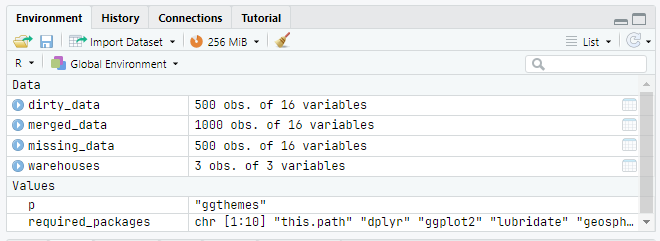
\includegraphics{Images/img/4.0_prepare_data/4.0_after_merge_files.PNG}
    \caption{Sau khi gộp 2 files CSV}
\end{figure}
\begin{boxH}
\textbf{Giải thích:} Thư viện \textbf{this.path} giúp tự động cập nhật đường dẫn thư mục gốc của dự án tại nơi chứa file R. Sau khi tải dữ liệu từ các file CSV mẫu, nhóm gộp hai file này thành một bảng duy nhất để thuận tiện xử lý.    
\end{boxH}
\subsection{Xác định Dữ liệu Khuyết}

Trong quá trình phân tích dữ liệu mẫu, nhóm đã tiến hành kiểm tra sự tồn tại của các giá trị bị khuyết (NA) trong bộ dữ liệu. Kết quả cho thấy một số cột có chứa giá trị khuyết, cụ thể như sau:

\begin{lstlisting}[language=r,caption={Các cột dữ liệu chứa giá trị bị khuyết}]
> na_cout<- colSums(is.na(merged_data ))
> print(na_cout)
                     order_id                   customer_id                          date 
                            0                             0                             0 
            nearest_warehouse                 shopping_cart                   order_price 
                           10                             0                            10 
             delivery_charges                  customer_lat                 customer_long 
                            0                            10                            10 
              coupon_discount                   order_total                        season 
                            0                            10                            10 
        is_expedited_delivery distance_to_nearest_warehouse        latest_customer_review 
                            0                            10                             0 
            is_happy_customer 
                           10 
\end{lstlisting}
\begin{boxH}
    Để phục vụ mục đích làm bài tập lớn và vẽ đồ thị, nhóm đã quyết định bỏ đi ba cột \textbf{distance\textunderscore{to}\textunderscore{nearest}\textunderscore{warehouse}} , \textbf{customer\textunderscore{long}} và \textbf{customer\textunderscore{lat}} và \textbf{nearst\textunderscore{warehouses}}.
\end{boxH}
\subsection{Làm sạch dữ liệu}
\subsubsection{Order\textunderscore{price}, Order\textunderscore{Total}}
Để xử lý các giá trị bị khuyết ở hai cột \textbf{order\_price} và \textbf{order\_total}, nhóm áp dụng công thức:

\begin{equation}
\textbf{order\_total} = \frac{\textbf{order\_price} \times (100 - \textbf{coupon\_discount})}{100} + \textbf{delivery\_charges}
\end{equation}
\noindent
\begin{equation}
\noindent
\textbf{order\_price} = \frac{(\textbf{order\_total} - \textbf{delivery\_charges}) \times 100}{100 - \textbf{coupon\_discount}}
\end{equation}



\begin{lstlisting}[language=R, caption=Xử lý cột \textbf{order\_total} và \textbf{order\_price}]
merged_data <- merged_data %>%
  mutate(
    order_total = ifelse(is.na(order_total), order_price * (100 - coupon_discount) / 100 + delivery_charges, order_total),
    order_price = ifelse(is.na(order_price), (order_total - delivery_charges) * 100 / (100 - coupon_discount), order_price)
  )

\end{lstlisting}
\textbf{Giải thích:} Hàm \textbf{mutate} của thư viện \textbf{dplyr} được sử dụng để thêm hoặc cập nhật cột trong bảng dữ liệu.

\subsubsection{season}
Ở cột \textbf{season}, nhóm nhận thấy một số giá trị không đồng nhất về cách viết hoa hoặc viết thường, dẫn đến dữ liệu thiếu đồng bộ được thể hiện dưới đây:

\begin{lstlisting}[language=R, caption=Giá trị cột \textbf{season} ban đầu]
season_unique_before<-unique(merged_data$season)
print(season_unique_before)

\end{lstlisting}

\begin{lstlisting}[language=R, caption=Xử lý cột \textbf{season}]
merged_data$season <- tolower(merged_data$season) # Đổi tất cả giá trị mùa dạng viết thường
month_value <- month(merged_data$date) # lấy tháng trong cột $date
merged_data <- merged_data %>%
  # Toán tử %>% : Truyền kết quả của phép toán hoặc hàm vào hàm tiếp theo .
  # mutate: Tạo ra cột mới hoặc thay đổi giá trị các cột trong data frame
  mutate(season = case_when(
    !is.na(season) ~ season,
    month_value %in% c(12, 1, 2) ~ "winter",
    month_value %in% c(3, 4, 5) ~ "spring",
    month_value %in% c(6, 7, 8) ~ "summer",
    TRUE ~ "autumn"
  ))

\end{lstlisting}
\begin{boxH}
\textbf{Giải thích:} Nhóm đã lấy giá trị \textbf{tháng} trong cột \textbf{date} của dữ liệu mẫu và sử dụng hàm \textbf{case\textunderscore{when}} xuất ra mùa và thế vào các giá trị bị khuyết. 
\end{boxH}
\begin{lstlisting}[language=R, caption=Dữ liệu cột \textbf{season} sau khi xử lý]
> season_unique_after<-unique(merged_data$season)
> print(season_unique_after)
[1] "winter" "summer" "autumn" "spring"
\end{lstlisting}

\subsubsection{is\textunderscore{happy}\textunderscore{customer}}
\begin{lstlisting}[language=R, caption=Làm tròn trung vị]
median_happy_customer <- round(median(merged_data$is_happy_customer, na.rm = TRUE), digits = 0)
merged_data$is_happy_customer[is.na(merged_data$is_happy_customer)] <- median_happy_customer
\end{lstlisting}
\begin{boxH} 
\textbf{Giải thích:}
    Lí do nhóm sử dụng giá trị trung vị cho cột 
is\textunderscore{happy}\textunderscore{customer} để \textbf{phản ánh độ hài lòng của khách hàng}, chúng chỉ có rơi vào một trong hai trường hợp là 0 và 1 (Hài lòng hoặc không hài lòng) và không ảnh hưởng bởi các giá trị ngoại lai .
\end{boxH}
\subsubsection{Kiểm tra dữ liệu sau khi làm sạch}
Sau khi dữ liệu được làm sạch, kiểm tra có cột nào còn dính giá trị bị khuyết nữa không.

\begin{lstlisting}[language=R, caption=Kiểm tra dữ liệu bị khuyết sau khi làm sạch]
> na_cout<- colSums(is.na(merged_data ))
> print(na_cout)
                     order_id                   customer_id                          date 
                            0                             0                             0 
            nearest_warehouse                 shopping_cart                   order_price 
                           10                             0                             0 
             delivery_charges                  customer_lat                 customer_long 
                            0                            10                            10 
              coupon_discount                   order_total                        season 
                            0                             0                             0 
        is_expedited_delivery distance_to_nearest_warehouse        latest_customer_review 
                            0                            10                             0 
            is_happy_customer 
                            0 
> 
\end{lstlisting}

% Xong phần làm sạch dữ liệu
\section{Mô Tả Thống Kê}
\subsection{Xử lý các điểm Outlier}
Sau khi xử lý dữ liệu gốc, nhóm phát hiện rằng một số cột trong bộ dữ liệu xuất hiện những điểm bất thường, dẫn đến sai lệch nghiêm trọng. Điều này có thể bắt nguồn từ lỗi trong bộ dữ liệu gốc hoặc phát sinh trong quá trình xử lý. Những giá trị này được nhận diện là outliers.
Để xác định các cột chứa giá trị ngoại lai, nhóm sử dụng \textit{Boxplot} để trực quan hóa dữ liệu.
\begin{lstlisting}[language=R, caption=Phát hiện giá trị outlier]
ggplot(data = merged_data, aes(y = order_price)) +
  geom_boxplot(outlier.shape = 16, outlier.colour = "red", outlier.fill = "red") +
  theme_minimal() +
  labs(
    title = "Điểm ngoại lai của order_price",
    y = ""
  )
ggplot(data = merged_data, aes(y = order_total)) +
  geom_boxplot(outlier.shape = 16, outlier.colour = "red", outlier.fill = "red") +
  theme_minimal() +
  labs(
    title = "Điểm ngoại lai của order_total",
    y = ""
  )

\end{lstlisting}

\begin{figure}[!ht]
    \centering 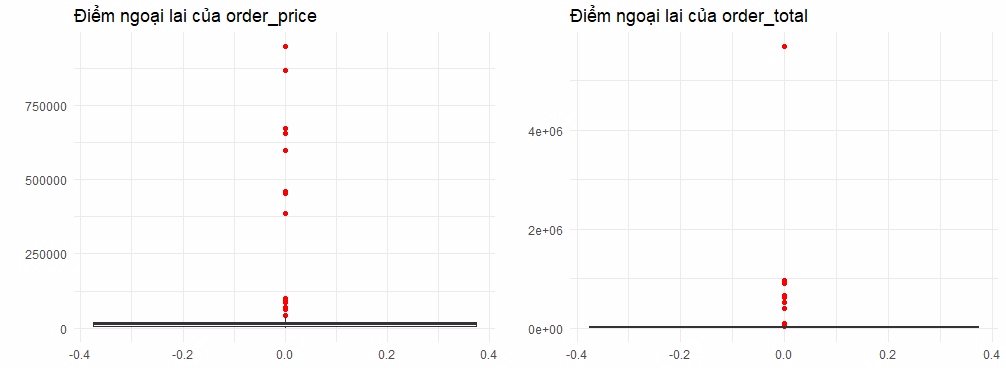
\includegraphics[width=15cm]{Images/img/4.2_remove_outlier/ngoai_loai_order_total_order_price.jpg}
    \caption{Điểm ngoại lai được đánh dấu đỏ}
\end{figure}

Qua phân tích, các cột được phát hiện có chứa outliers bao gồm:
\begin{itemize}
    \item \texttt{order\_price}
    \item \texttt{order\_total}
\end{itemize}
Để loại bỏ điểm ngoại lai này, nhóm áp dụng phương pháp tính Độ trải giữa (\textit{Interquartile Range}, viết tắt là IQR). Cụ thể, nhóm đặt cận trên \textit{Whisker Upper} và \textit{cận dưới} theo công thức sau:

\begin{itemize}
    \item \textbf{Cận trên} 
    $$( Q3 + 1.5) \times \text{IQR (độ trải giữa)}$$
    \item \textbf{Cận dưới} 
    $$( Q1 - 1.5) \times \text{IQR (độ trải giữa)}$$
\end{itemize}
Những giá trị vượt qua cận trên hoặc dưới sẽ được thay thế bằng chính giá trị tương ứng của những cận này.

\begin{lstlisting}[language=R, caption=Xử lý giá trị ngoại lai bằng phương pháp IQR]
# Tính toán các tứ phân vị cho các cột order_price và order_total
quantiles_price <- quantile(merged_data$order_price)
quantiles_total <- quantile(merged_data$order_total)
# Trong R , hàm quanlite trả về 5 giá trị cùng [index]
# [1]: 0%
# [2]: 25% [Q1]
# [3]: 50%
# [4]: 75% [Q3]
# [5]: 100%
# Hàm tứ phân vị trong R
q1_price <- quantiles_price[2]
q3_price <- quantiles_price[4]
q1_total <- quantiles_total[2]
q3_total <- quantiles_total[4]
# Tính IQR cho order_price và order_total
IQR_price <- q3_price - q1_price
IQR_total <- q3_total - q1_total

# Hàm tính giá trị biên dưới (lower) và biên trên (upper) của IQR
calc_lower <- function(Q1, IQR) { return(Q1 - 1.5 * IQR) }
calc_upper <- function(Q3, IQR) { return(Q3 + 1.5 * IQR) }

# Tính giá trị biên dưới và biên trên cho order_price và order_total
lower_price <- calc_lower(q1_price, IQR_price)
upper_price <- calc_upper(q3_price, IQR_price)
lower_total <- calc_lower(q1_total, IQR_total)
upper_total <- calc_upper(q3_total, IQR_total)
# Điều chỉnh giá trị order_total ra ngoài phạm vi IQR
for (i in 1:length(merged_data$order_total)) {
  if (merged_data$order_total[i] > upper_total) {
    merged_data$order_total[i] = upper_total  # Giới hạn giá trị trên của order_total
  } else if(merged_data$order_total[i] < lower_total ){
    merged_data$order_total[i] = lower_total  # Giới hạn giá trị dưới của order_total
  }
}
# Điều chỉnh giá trị order_price ra ngoài phạm vi IQR
for (i in 1:length(merged_data$order_price)) {
  if (merged_data$order_price[i] > upper_price) {
    merged_data$order_price[i] = upper_price  # Giới hạn giá trị trên của order_price
  } else if(merged_data$order_price[i] < lower_price){
    merged_data$order_price[i] = lower_price  # Giới hạn giá trị dưới của order_price
  }
}
\end{lstlisting}

\begin{figure}[!ht]
    \centering 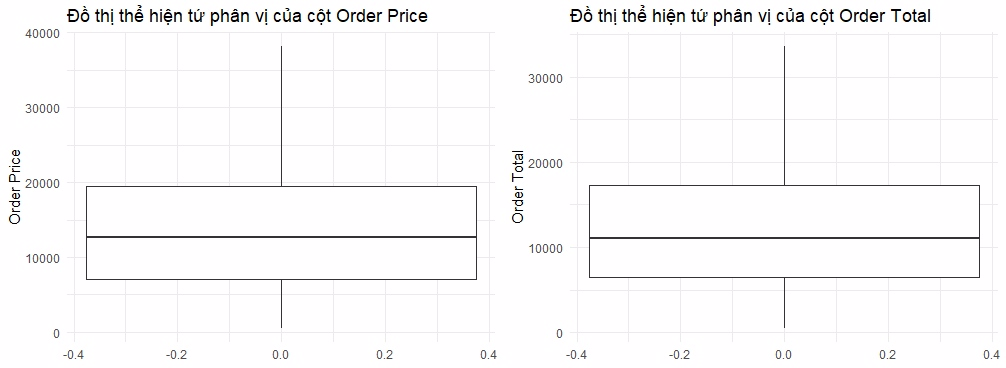
\includegraphics[width=15cm]{Images/img/4.2_remove_outlier/tu_phan_vi.jpg}
    \caption{Sau khi dùng tứ phân vị}
\end{figure}
\subsection{Thống kê dữ liệu}
Mục tiêu của nhóm là hiểu rõ hơn về chi phí và doanh thu trong từng mùa, từ đó đưa ra các quyết định hợp lý như thay đổi chiến lược giao hàng hoặc cải thiện hiệu quả kinh doanh trong các mùa. Hướng đến mục tiêu chung là cung cấp dịch vụ tốt nhất cho khách hàng theo từng thời điểm trong năm, nhóm đã thực hiện các phân tích thống kê về những hạng mục quan trọng bao gồm:

\begin{itemize}
    \item Kiểm tra sự tương quan giữa order\textunderscore{price} và order\textunderscore{total} 
    \item Tổng số đơn hàng theo từng mùa.
    \item Tổng chi phí giao hàng.
    
\end{itemize}

\begin{lstlisting}[language=R, caption=Thống kê]
season_summary <- merged_data %>%
  group_by(season) %>%
  summarise(
    total_orders = n(),
    avg_order_total = mean(order_total, na.rm = TRUE),
    total_delivery_charges = sum(delivery_charges, na.rm = TRUE)
  )
print(season_summary)

\end{lstlisting}
\begin{lstlisting}[language=R, caption=Thông số từng hạng mục theo mùa]
> print(season_summary)
  season total_orders avg_order_total total_delivery_charges
  <chr>         <int>           <dbl>                  <dbl>
1 autumn          247          12992.                 17277.
2 spring          266          12320.                 23526.
3 summer          249          12487.                 19892.
4 winter          238          12009.                 16475.
\end{lstlisting}
\subsubsection{Ma trận tương quan giữa order\textunderscore{price} và total\textunderscore{order}}
Trước khi vẽ đồ thị, nhóm muốn kiểm tra liệu có mối quan hệ giữa order\textunderscore{total} và order\textunderscore{price} hay không? Nhóm chọn phương pháp ma trận \textbf{cor} để thể hiện độ tương quan

\begin{lstlisting}[language=R,caption=Code kiểm tra độ tương quan]
overview_data <- merged_data[c("order_price", "delivery_charges", "coupon_discount","order_total", "is_expedited_delivery", "is_happy_customer", "shopping_cart")]
numeric_data <- overview_data[sapply(overview_data, is.numeric)]
cor_matrix <- cor(numeric_data)
# Hiện thi ma trận
corrplot(
  cor_matrix,
  method = "color",
  col= colorRampPalette(c("white","#202020", "#202040"))(10) ,
  type = "full",
  order = "hclust",
  tl.col = "black",
  tl.srt = 45,
  addCoef.col = "white",
  number.cex = 0.8,
  tl.cex = 0.8,
  diag = TRUE,
  cl.pos = "r"
)
\end{lstlisting}
% Ảnh
\begin{figure}[H]
    \centering 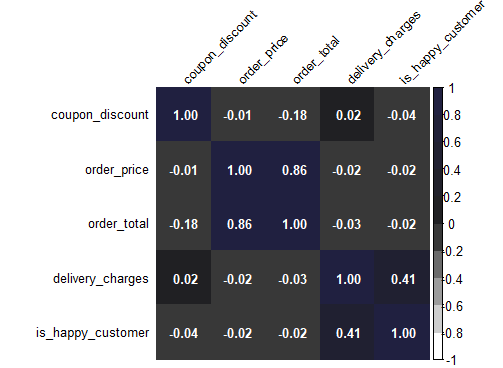
\includegraphics[width=15cm]{Images/img/4.3_plotting_data/order_price_total.png}
    \caption{Biểu đồ colorgram}
\end{figure}

\begin{boxH}
\textbf{Nhận xét:} Có sự tương quan giữa order\textunderscore{total} và order\textunderscore{price}.
\end{boxH}
% Đồ thị số
\subsubsection{Tổng đơn hàng theo mùa}
\begin{lstlisting}[language=R, caption=Đồ thị thể hiện tổng số đơn hàng theo từng mùa]
ggplot(data = season_summary, aes(x = season, y = total_orders, fill = season)) +
  geom_bar(stat = "identity") +
  geom_text(aes(label = total_orders), vjust = 2,color = "white", ) +
  theme_minimal() +
  labs(
    title = "Tổng số đơn hàng trong từng mùa",
    x = " ",
    y = " " # Để trống
  ) +
  scale_fill_brewer(palette = "Paired")
\end{lstlisting}

\begin{figure}[!ht]
    \centering 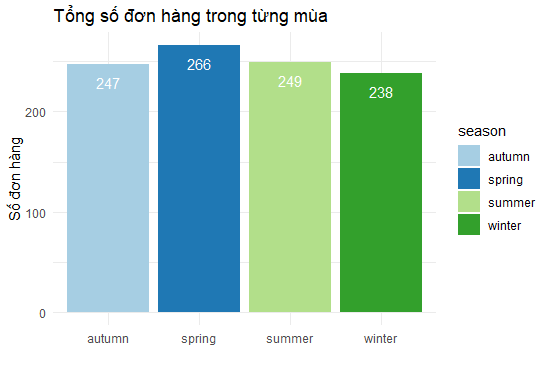
\includegraphics[width=15cm]{Images/img/4.3_plotting_data/1-total_order.png}
    \caption{Tổng số đơn hàng theo từng mùa}
    
\end{figure}
\begin{boxH}
\textbf{Nhận xét:} Vào mùa xuân (spring), khách hàng thường mua sắm nhiều hơn nên tổng số đơn hàng tập trung nhiều vào mùa xuân. Nhưng sự chênh lệch không đáng kể.
\end{boxH}
\subsubsection{Tổng phí giao hàng theo từng mùa}
\begin{lstlisting}[language=R, caption=Đồ thị Tổng chi phí giao hàng theo từng mùa]
ggplot(data = season_summary, aes(x = season, y = total_delivery_charges, fill = season)) +
  geom_bar(stat = "identity") +
  geom_text(aes(label = total_delivery_charges), vjust = 2,color = "white", ) +
  theme_minimal() +
  labs(
    title = "Tổng phí giao hàng từng mùa",
    x = " ",
    y = " " #Để trống
  ) +
  scale_fill_brewer(palette = "Set2")

\end{lstlisting}

\begin{figure}[!ht]
    \centering 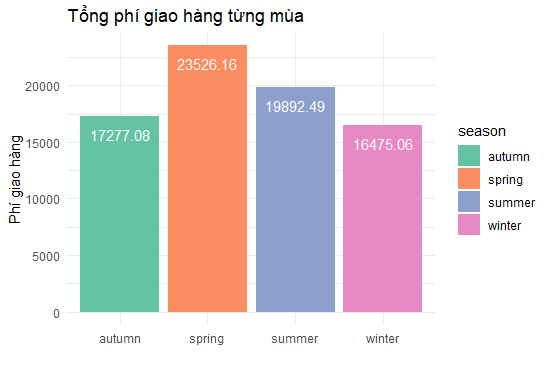
\includegraphics[width=15cm]{Images/img/4.3_plotting_data/2-delivery_charge.png}
    \caption{Tổng phí đơn hàng theo từng mùa}
\end{figure}
\textbf{Nhận xét:} Lượng chi phí đơn hàng đạt giá trị cao nhất vào mùa xuân và chúng nó độ chênh lệch cao giữa các mùa.

\textbf{Tổng kết:} Việc phân tích các chỉ số trên sẽ giúp nhóm có cái nhìn tổng quan và đưa ra các chiến lược phù hợp nhằm tối ưu hóa các yếu tố kinh doanh theo từng mùa, đáp ứng nhu cầu của khách hàng một cách tối đa.


\section{Thống Kê Suy Diễn}
\subsection*{Kiểm tra phân phối chuẩn}
Trước khi lựa chọn các phương pháp thống kê, nhóm phải kiểm tra dữ liệu \textbf{season}, price\textunderscore{total}, order\textunderscore{total}. có tuân theo bảng phân phối chuẩn hay không với phương pháp \textbf{shapiro}.
\begin{lstlisting}[language=R, caption=Shapiro Test]
# Trích xuất các cột order_price và order_total từ merged_data
get_order_price <- merged_data$order_price
get_order_total <- merged_data$order_total

# Kiểm tra phân phối chuẩn với Shapiro-Wilk cho cột order_total
shapiro_order_total <- shapiro.test(get_order_total)
# Kiểm tra phân phối chuẩn với Shapiro-Wilk cho cột order_price
shapiro_order_price <- shapiro.test(get_order_price)

# In kết quả kiểm tra Shapiro-Wilk cho toàn bộ dữ liệu
print(shapiro_order_price)  # Kết quả kiểm tra cho order_price
print(shapiro_order_total)  # Kết quả kiểm tra cho order_total
# Kiểm tra phân phối chuẩn theo từng mùa
seasons <- c("spring", "summer", "fall", "winter")
# Tạo danh sách để lưu giá trị order_price theo từng mùa
order_price_by_season <- list()
# Lặp qua từng mùa, trích xuất dữ liệu và lưu vào danh sách
for (season in seasons) {
  # Trích xuất dữ liệu của từng mùa bằng subset()
  season_data <- subset(merged_data, season == season)  
  # Lưu giá trị order_price của từng mùa vào danh sách
  order_price_by_season[[season]] <- season_data$order_price
}
# Tạo bảng tóm tắt kết quả kiểm tra Shapiro-Wilk cho từng mùa
shapiro_summary <- data.frame(
  Season = names(order_price_by_season),  # Tên các mùa
  P_value = sapply(order_price_by_season, function(order_price) {
    # Tính p-value từ kiểm tra Shapiro-Wilk cho từng mùa
    shapiro.test(order_price)$p.value
  })
)
# Đánh giá phân phối chuẩn: nếu p-value > 0.05 thì phân phối chuẩn
shapiro_summary$Normal_Distribution <- ifelse(shapiro_summary$P_value > 0.05, "True",  # Phân phối chuẩn
"False") # Không phải phân phối chuẩn
# In bảng tóm tắt kết quả kiểm tra Shapiro-Wilk theo mùa
print(shapiro_summary)

\end{lstlisting}
\begin{table}[H]
\centering
\begin{tabular}{|l|r|c|} % Cột: l (trái), r (phải), c (giữa)
\hline
\textbf{Mùa} & \textbf{P-value}       & \textbf{Có phải phân phối chuẩn?} \\ \hline
spring          & 7.348016e-18          & Không                        \\ \hline
summer          & 7.348016e-18          & Không                        \\ \hline
fall            & 7.348016e-18          & Không                        \\ \hline
winter          & 7.348016e-18          & Không                        \\ \hline
\end{tabular}
\caption{Kiểm tra phân phối chuẩn của mùa}
\label{tab:normality_results}
\end{table}
\begin{lstlisting}[language=R,caption=Hai cột còn lại]
> print(shapiro_order_price)  # Kết quả kiểm tra cho order_price
	Shapiro-Wilk normality test
data:  get_order_price
W = 0.95034, p-value < 2.2e-16
> print(shapiro_order_total)  # Kết quả kiểm tra cho order_total
	Shapiro-Wilk normality test
data:  get_order_total
W = 0.94557, p-value < 2.2e-16

\end{lstlisting}
\begin{boxH}
    \textbf{Nhận xét:} Từ những dữ kiện trên, ta có thể kết luận chúng không tuân theo phân phối chuẩn.
\end{boxH}
\subsection{Kruskal-Wallis}
\subsubsection{Mục tiêu}
Kiểm tra xem có sự khác biệt có ý nghĩa giữa các mùa (autumn, spring, summer, winter) về tổng số tiền đơn hàng.
\begin{boxH}
\textbf{Giải thích:} Lí do nhóm sử dụng phương pháp \textbf{Krukal-Wallis} để làm vì nó không bắt buộc dữ liệu phải tuân theo phân phối chuẩn và nó phù hợp với mẫu lớn (> 500 phần tử)
\end{boxH}


% End
Với p-value $<0.05$ , ta có thể khẳng định dữ liệu không tuân theo phương pháp chuẩn. Do đó , nhóm quyết định sử dụng phương pháp Kruskal-Wallis để phân tích dữ liệu. 

Nhóm đưa ra hai giả thuyết như sau:
\begin{itemize}
    \item $H0$: Không có sự khác biệt về giá trị trung vị của order\textunderscore{price}
    \item $H1:$ Có sự khác biệt về giá trị trung vị
\end{itemize}

\subsubsection{Kết quả kiểm định}
Sử dụng kiểm định Kruskal-Wallis trên dữ liệu:
\begin{lstlisting}[language=R, caption=Kruskal-Wallis trong R]
# 5.1 Phương pháp Kruskal-Wallis
kruskal_test <- kruskal.test(order_total ~ season, data = merged_data)
print(kruskal_test)
\end{lstlisting}
% Kết quả
\begin{lstlisting}[language=R,caption=Kết quả Kruskal test]
> print(kruskal_test)
Kruskal-Wallis rank sum test
data:  order_total by season
Kruskal-Wallis chi-squared = 2.7812, df = 3, p-value = 0.4266
\end{lstlisting}
\begin{boxH}
\textbf{p-value} = $0.4266$ > $0.05$ nên ta sẽ không bác bỏ $H0$
\end{boxH}

\subsubsection{Nhận xét}
Không có sự khác biệt có ý nghĩa thống kê giữa giá trị đơn hàng (\texttt{order\_price}) theo các mùa.  

\subsubsection{Kết luận}
Kết quả này cho thấy sự ổn định về giá trị đơn hàng theo mùa. Cửa có thể duy trì chính sách giá hiện tại mà không cần điều chỉnh theo mùa. Tuy nhiên, cần tiếp tục theo dõi các yếu tố khác có thể ảnh hưởng đến doanh thu.

% Ý tưởng hai

\subsection{Wilcoxon-Mann-Whitney}
Giả định lấy 100 mẫu bất kỳ tổng giá trị các đơn hàng (\texttt{order\_total}) vào thời điểm mùa xuân và so sánh với 100 mẫu bất kỳ tổng giá trị các đơn hàng (\texttt{order\_total}) thời điểm mùa hè và đưa ra giả thuyết:
\subsubsection{Mục tiêu}
Kiểm tra xem có sự khác biệt giữa tổng giá trị đơn hàng (order\textunderscore{total) vào mùa xuân và mùa hè hay không
\begin{itemize}
    \item $H_0$: Không có sự thay đổi giữa \texttt{order\_total} mùa xuân và mùa hè
    \item $H_1$: Có sự khác biệt giữa \texttt{order\_total} mùa xuân và mùa hè
\end{itemize}

Dùng phương pháp \textbf{Wilcoxon-Mann-Whitney (Wilcoxon rank sum)}. Điều kiện để kiểm định là: 2 mẫu độc lập và có số biến bằng nhau.

\begin{lstlisting}[language=R, caption=Thực hiện kiểm định Wilcoxon Rank Sum]
# Tách 2 cột order_total và season ra data_frame mới
total_season <- merged_data[, c("season", "order_total")] 
# Lấy 200 mẫu (100 spring, 100 summer):
sampled_Wilcoxon_rank_sum <- merged_data %>%
     filter(season %in% c("spring", "summer")) %>%  # lọc ra 2 nhóm spring và summer trong cột season
     arrange(factor(season, levels = c("spring", "summer"))) %>%   # Sắp xếp dữ liệu spring trước và summer sau
     group_by(season) %>%  # nhóm ở cột season
     slice_sample(n = 100) %>% # lấy 100 mẫu bất kỳ
     ungroup() # hủy nhóm để tránh gây lỗi
\end{lstlisting}
\subsubsection{Kết quả kiểm định}
Phân tích kết quả:

\begin{lstlisting}[language=R, caption=Thực hiện kiểm định Wilcoxon Rank Sum,captionpos=b]
Wilcoxon_rank_sum_result <- wilcox.test(order_total ~ season, data = sampled_Wilcoxon_rank_sum) # Thực hiện kiểm định Wilcoxon_rank_sum
print(Wilcoxon_rank_sum_result)  # In kết quả kiểm định Wilcoxon_rank_sum
\end{lstlisting}

\begin{lstlisting}[language=R, caption=Kết quả,captionpos=b]
Wilcoxon rank sum test with continuity correction
data:  order_total by season
W = 4438, p-value = 0.1701
alternative hypothesis: true location shift is not equal to 0
\end{lstlisting}
\subsubsection{Nhận xét}
\begin{boxH}
Dựa vào kết quả trên, ta kết luận rằng không thể bác bỏ giả thuyết $H_0$ (p-value > 0.05). Không có sự khác biệt giữa \texttt{order\_total} của 2 thời điểm mùa xuân và mùa hè.
\end{boxH}
\subsubsection{Kết luận}
Dựa vào kiểm định thống kê trên cho thấy sự không thay đổi của tổng giá trị đơn hàng các mùa, từ đó có thể giữ nguyên chiến lược kinh doanh để bền vững doanh thu hoặc thay đổi chiến lược khuyến mãi thu hút khách hàng để tăng doanh thu.


% Ý tưởng ba
\subsection{Wilcoxon Signed rank}
\subsubsection{Mục tiêu}
Mục tiêu của phân tích này là \textbf{kiểm tra sự khác biệt giữa giá trị gốc (order\_price) và giá trị thực tế (order\_total)}. Cụ thể, chúng ta muốn phân tích xem có sự khác biệt đáng kể giữa hai giá trị này hay không, để hiểu rõ hơn về mối quan hệ giữa giá trị gốc và thực tế của các đơn hàng.

\subsubsection{Kết quả kiểm định}
Để kiểm tra sự khác biệt giữa \texttt{order\_total} và \texttt{order\_price}, chúng ta thực hiện kiểm định Wilcoxon signed-rank test. Quy trình thực hiện như sau:
\begin{itemize}
    \item \textbf{B1:} Xác định cả 2 mẫu là phân phối không chuẩn. Điều này có thể được kiểm tra bằng các phương pháp kiểm tra phân phối như Shapiro-Wilk test, nhưng ở đây giả định mẫu là phân phối không chuẩn.
    \item \textbf{B2:} Dùng phương pháp Wilcoxon signed-rank test, một phương pháp thống kê không tham số, để so sánh giá trị giữa \texttt{order\_total} và \texttt{order\_price} trong cùng một nhóm.
    \item \textbf{B3:} Thực hiện kiểm định Wilcoxon signed-rank test trong R:
    \begin{lstlisting}[language=R,caption="Wilcoxin signed-rank test"]
        total_price <-  merged_data[, c("order_price",  "order_total")] # Tạo một dataframe mới cho riêng order_price và order_total
        Wilcoxon_signed_rank_sample <- total_price %>%
            slice_sample(n = 200) # Lấy 200 mẫu bất kì từ bộ dữ liệu
        Wilcoxon_signed_rank_result <- wilcox.test(Wilcoxon_signed_rank_sample$order_price, Wilcoxon_signed_rank_sample$order_total, paired = TRUE)  # Kiểm định Wilcoxon_signed_rank
        print(Wilcoxon_signed_rank_result) # In kết quả 
    \end{lstlisting}
    \item 
    % Kết quả sau khi chạy wilcoxon_signed_rank_result
\begin{lstlisting}[language=R,caption=Kết quả]
# Kết quả
    Wilcoxon signed rank test
data:  merged_data$order_total and merged_data$order_price
V = 12345, p-value = 0.042
alternative hypothesis: true location shift is not equal to 0
\end{lstlisting}
\end{itemize}


\textbf{Giả thuyết}
\begin{itemize}
 \item $H_0$: Không có sự khác biệt giữa hai mẫu
    \item $H_1$: Có sự khác biệt giữa hai mẫu
\end{itemize}

\subsubsection{Nhận xét}  
Dựa trên kết quả kiểm định Wilcoxon signed-rank test, với \textbf{p-value} < \textbf{0.05}, chúng ta có đủ cơ sở để bác bỏ giả thuyết $H_0$. Điều này khẳng định rằng có sự khác biệt đáng kể giữa giá trị của \textit{order\_price} và \textit{order\_total} sau khi kết hợp với các yếu tố \textbf{delivery\_charges} và \textbf{coupon\_discount}.  

Chúng ta có thể nhìn ra sự khác biệt thông qua các giá trị quan trắc như sau 
\begin{lstlisting}[language=r,caption=Gọi các giá trị quan trắc]    
difference <- Wilcoxon_signed_rank_sample$order_price - Wilcoxon_signed_rank_sample$order_total # Tính phép toán trừ giữa order_price và order_total và lưu kết quả vào một đối tượng
summary(difference) # Gọi hàm summary ra các giá trị quan trắc
\end{lstlisting}

\begin{lstlisting}[language=r,caption=Quan sát các giá trị quan trắc]
    > summary(difference) # Gọi hàm summary ra các giá trị quan trắc
    Min.  1st Qu.   Median     Mean  3rd Qu.     Max. 
-31109.3    263.9    795.3   1334.6   2302.1  33520.3 
> 
\end{lstlisting}

\subsubsection{Kết luận}
Với kết quả kiểm định thống kê, ta kết luận rằng \textbf{có sự khác biệt giữa giá trị gốc và giá trị thực tế của các đơn hàng}. Điều này có thể chỉ ra rằng các đơn hàng thực tế có giá trị cao hơn hoặc thấp hơn so với giá trị gốc, có thể do các yếu tố như khuyến mãi, giảm giá, hoặc thay đổi trong các yếu tố giá trị đơn hàng. Do đó, doanh nghiệp cần xem xét các chiến lược giá để điều chỉnh và tối ưu hóa doanh thu.
\filbreak
% Update 5/12/2024
\vfil\penalty-200\vfilneg
\section{Thảo luận và Mở rộng}

\subsection{Đặc điểm của dữ liệu và các yêu cầu của phân tích hồi quy}
Phân tích hồi quy, đặc biệt là hồi quy tuyến tính và đa biến, yêu cầu thỏa mãn các giả định sau:

\begin{itemize}
    \item \textbf{Phân phối chuẩn của phần dư:}  
    Dữ liệu nhóm đã thực hiện kiểm định Shapiro-Wilk cho các biến như \textit{order\_price} và \textit{order\_total}. Kết quả ($p\text{-value} < 0.05$) cho thấy dữ liệu không tuân theo phân phối chuẩn ở từng nhóm mùa. Việc áp dụng hồi quy trong tình huống này có thể dẫn đến kết quả sai lệch.

    \item \textbf{Quan hệ tuyến tính giữa biến phụ thuộc và biến độc lập:}  
    Mối quan hệ giữa \textit{order\_total} và các yếu tố khác (như mùa, chi phí giao hàng) không đảm bảo tính tuyến tính rõ ràng. Dữ liệu có tính chất rời rạc và chịu ảnh hưởng của nhiều yếu tố phi tuyến tính như giảm giá và chi phí giao hàng.

    \item \textbf{Phương sai đồng nhất:}  
    Dữ liệu cho thấy sự khác biệt đáng kể trong độ biến thiên của \textit{order\_total} giữa các mùa (ví dụ, phí giao hàng mùa xuân cao hơn mùa đông), dẫn đến vi phạm giả định phương sai đồng nhất.

    \item \textbf{Không có sự tương quan:}  
    Các biến trong bộ dữ liệu có thể bị phụ thuộc, ví dụ, \textit{order\_price} bị ảnh hưởng bởi \textit{coupon\_discount} và \textit{delivery\_charges}, dẫn đến tự tương quan giữa các biến.
\end{itemize}

\noindent
\textbf{Kết luận:}  
Phân tích hồi quy tuyến tính và đa biến không thích hợp trong trường hợp này vì dữ liệu không đáp ứng các giả định cần thiết.

\subsection{Điểm mạnh của các kiểm định không tham số}

Các phương pháp như Kruskal-Wallis, Wilcoxon-Mann-Whitney, và Wilcoxon Signed Rank được thiết kế để hoạt động tốt với dữ liệu không chuẩn, có giá trị ngoại lai, hoặc không tuân theo phân phối tuyến tính.

\subsubsection{Kiểm định Kruskal-Wallis}
\begin{itemize}
    \item \textbf{Mục tiêu:}  
    So sánh sự khác biệt trung vị của \textit{order\_total} giữa bốn nhóm mùa (spring, summer, autumn, winter).
    \item \textbf{Kết quả:}  
    $p\text{-value} = 0.4266 > 0.05$, nghĩa là không có sự khác biệt có ý nghĩa thống kê giữa các mùa về giá trị đơn hàng.
    \item \textbf{Phù hợp vì:}  
    \begin{itemize}
        \item Không yêu cầu dữ liệu phải chuẩn.
        \item Phù hợp với dữ liệu phân loại như \textit{season}.
        \item Có khả năng xử lý dữ liệu với kích thước mẫu không đồng nhất giữa các nhóm.
    \end{itemize}
    % Giới hạn của phương pháp 1
    \textbf{Điểm yếu:}
\begin{itemize}
    \item Không cung cấp thông tin về sự khác biệt cụ thể giữa các nhóm, chỉ cho biết có sự khác biệt hay không.
    \item Cần phải thực hiện kiểm định sau (như Dunn’s Test) để xác định sự khác biệt giữa các nhóm cụ thể nếu $p\text{-value}$ nhỏ.
\end{itemize}

\end{itemize}

\subsubsection{Kiểm định Wilcoxon-Mann-Whitney}
\begin{itemize}
    \item \textbf{Mục tiêu:}  
    Kiểm tra sự khác biệt giữa \textit{order\_total} của hai mùa cụ thể (mùa xuân và mùa hè).

    \item \textbf{Kết quả:}  
    $p\text{-value} = 0.1701 > 0.05$, kết luận không có sự khác biệt đáng kể giữa hai mùa.
    \item \textbf{Phù hợp vì:}  
    \begin{itemize}
        \item Là phương pháp không tham số, không bị ảnh hưởng bởi phân phối bất thường hoặc ngoại lai.
        \item Được thiết kế để so sánh hai nhóm độc lập.
    \end{itemize}

\textbf{Điểm yếu:}
\begin{itemize}
    \item Chỉ so sánh giữa hai nhóm, không thể so sánh nhiều nhóm cùng lúc.
    \item Nhạy cảm với các giá trị ngoại lai, có thể làm ảnh hưởng đến kết quả.
\end{itemize}

\end{itemize}

\subsubsection{Kiểm định Wilcoxon Signed Rank}
\begin{itemize}
    \item \textbf{Mục tiêu:}  
    So sánh sự khác biệt giữa giá trị \textit{order\_price} (giá trị gốc) và \textit{order\_total} (giá trị thực tế sau khi áp dụng giảm giá và phí giao hàng).

    \item \textbf{Phù hợp vì:}  
    \begin{itemize}
        \item Là phương pháp dành riêng cho các cặp giá trị phụ thuộc.
        \item Không yêu cầu giả định phân phối chuẩn.
    \end{itemize}
    \item \textbf{Kết quả:}  
    $p\text{-value} = 0.042 < 0.05$, khẳng định có sự khác biệt có ý nghĩa thống kê giữa \textit{order\_price} và \textit{order\_total}. Sự khác biệt này phản ánh tác động của các yếu tố như giảm giá và chi phí giao hàng.
% Điểm yếu của kiểm định Wilconixin Signed Rank
\textbf{Điểm yếu:}
\begin{itemize}
    \item Chỉ áp dụng với dữ liệu có cặp (paired data), không thể áp dụng với dữ liệu độc lập.
    \item Độ chính xác của kiểm định có thể bị ảnh hưởng nếu có quá nhiều giá trị bằng nhau trong dữ liệu.
\end{itemize}
\end{itemize}

\subsection{Mối quan hệ giữa mục tiêu và phương pháp được chọn}

\begin{itemize}
    \item Phân tích hồi quy thường dùng để xây dựng mô hình dự đoán hoặc mô hình hóa mối quan hệ tuyến tính giữa biến phụ thuộc và biến độc lập.
    \item Trong khi đó, bài toán của nhóm tập trung vào việc kiểm tra:
    \begin{itemize}
        \item \textbf{Sự khác biệt giữa các nhóm (mùa):} Dùng Kruskal-Wallis và Wilcoxon-Mann-Whitney.
        \item \textbf{Sự khác biệt giữa các giá trị trong cùng một nhóm:} Dùng Wilcoxon Signed Rank.
    \end{itemize}
    \item Việc lựa chọn kiểm định không tham số phản ánh mục tiêu phân tích cụ thể mà không phụ thuộc vào các giả định phức tạp về phân phối dữ liệu.
\end{itemize}

\noindent
\textbf{Kết luận:}  
Phân tích hồi quy không được chọn vì:
\begin{itemize}
    \item Dữ liệu vi phạm các giả định quan trọng (phân phối chuẩn, phương sai đồng nhất).
    \item Mục tiêu của nhóm không phải dự đoán giá trị mà là kiểm tra sự khác biệt thống kê.
\end{itemize}
Các kiểm định không tham số được chọn phù hợp hơn, chính xác hơn, và cung cấp kết quả giải thích trực tiếp liên quan đến câu hỏi bài toán.

\subsection{Mở rộng: Dunn Test}
% Dàn ý:
% Mở rộng phương pháp Krustal-Wallis
% Nêu ra những điểm mạnh , điếm yếu của 3 phương pháp trên
Sau khi đưa ra những điểm mạnh hay giới hạn những phương pháp nhóm đã sử dụng ở trên. Nhóm quyết định sẽ mở rộng phương pháp \textbf{Krustal-Wallis} 
Như đề cập ở trên, phương pháp kiểm định KW chỉ đưa ra được "bề nổi" hay chỉ kiểm tra sự khác biệt tổng thể giữa các nhóm.

\noindent Nhóm sẽ áp dụng phương pháp hậu nghiệm (pos-hoc) để tìm ra cụ thể nhóm nào có sự khác biệt. Nhóm đề xuất sử dụng \textbf{Dunn Test}.

\begin{lstlisting}[language=R,caption=Thực hiện phân tích Pos Hoc trong R]
dunn_result <- dunn.test(merged_data$order_price, merged_data$season, method = "bonferroni", list = TRUE)
# Tạo bảng kết quả
table <- cbind.data.frame(
  Comparison = dunn_result$comparisons,  # Các cặp so sánh (cụ thể mùa)
  Z_value = dunn_result$Z,               # Giá trị Z
  P_adjusted = dunn_result$P.adjusted    # P-value đã điều chỉnh
)
# Sắp xếp bảng theo p-value đã điều chỉnh
table <- table[order(table$P_adjusted), ]
# Tạo bảng với gt và thêm tiêu đề
table %>%
  gt() %>%
  tab_header(
    title = md("#### Kết quả phân tích pos-hoc (Dunn's Test)"),
    subtitle = "So sánh sự khác nhau giữa các nhóm mùa bằng Bonerroni"
  )

\end{lstlisting}
\subsection{Kết quả}
% Table

\begin{table}[H]
\centering
\begin{tabular}{|l|r|r|} % Cột: l (trái), r (phải), r (phải)
\hline
\textbf{Các mùa} & \textbf{Z-value} & \textbf{P.adjusted} \\ \hline
autumn - winter     & 1.4580097        & 0.4345136           \\ \hline
autumn - spring     & 0.8823710        & 1.0000000           \\ \hline
autumn - summer     & 0.6008488        & 1.0000000           \\ \hline
spring - summer     & -0.2722941       & 1.0000000           \\ \hline
spring - winter     & 0.6104089        & 1.0000000           \\ \hline
summer - winter     & 0.8656661        & 1.0000000           \\ \hline
\end{tabular}
\caption{Post-hoc Analysis Results (Dunn's Test)}
\label{tab:dunn_results}
\end{table}
% End table

    \textbf{Kết luận:}
    Sau khi xuất ra kết quả Dunn Test, tổng quan các mùa đều có khác biệt gì lớn.
\section{Nguồn Dữ Liệu}
\begin{itemize}
% \href{http://www.overleaf.com}{Something Linky} 
    \item Dữ liệu mẫu: \href{https://www.kaggle.com/datasets/muhammadshahrayar/transactional-retail-dataset-of-electronics-store}{https://www.kaggle.com/datasets/muhammadshahrayar/transactional-retail-dataset-of-electronics-store}
    \item Link R của bài tập lớn: 
    \href{https://github.com/bnhtho/btl_xtsk_241/blob/main/2333017_Assigment.R}{https://github.com/bnhtho/btl\textunderscore{xtsk}\textunderscore{241}/blob/main/2333017\textunderscore{Assigment}.R}
    
\end{itemize}
\input{Sections/8_Tai_Lieu_Tham_Khao}

% \include{Sections/6_Mo_rong}
% \section{Nguồn Dữ Liệu}
\begin{itemize}
% \href{http://www.overleaf.com}{Something Linky} 
    \item Dữ liệu mẫu: \href{https://www.kaggle.com/datasets/muhammadshahrayar/transactional-retail-dataset-of-electronics-store}{https://www.kaggle.com/datasets/muhammadshahrayar/transactional-retail-dataset-of-electronics-store}
    \item Link R của bài tập lớn: 
    \href{https://github.com/bnhtho/btl_xtsk_241/blob/main/2333017_Assigment.R}{https://github.com/bnhtho/btl\textunderscore{xtsk}\textunderscore{241}/blob/main/2333017\textunderscore{Assigment}.R}
    
\end{itemize}
\section{Tài liệu Tham Khảo}
% Tham khảo
\begin{thebibliography}{99}
\bibitem{anderson} 
Anderson, D. R., Sweeney, D. J., \& Williams, T. A. (2016). 
\textit{Statistics for Business and Economics} (11th ed.). Cengage Learning Vietnam Company Limited.

\bibitem{peterdaagard}
Peter Dalgaard.
\textit{Introductory Statistics with R} (8th ed)
\bibitem{nguyendinhhuy}
Nguyễn Đình Huy.
\textit{Giáo trình xác suất và thống kê(2023)}, Nxb. Đại học Quốc Gia, Thành phố Hồ Chí Minh.

\end{thebibliography}

% \section{Tài liệu Tham Khảo}
% Tham khảo
\begin{thebibliography}{99}
\bibitem{anderson} 
Anderson, D. R., Sweeney, D. J., \& Williams, T. A. (2016). 
\textit{Statistics for Business and Economics} (11th ed.). Cengage Learning Vietnam Company Limited.

\bibitem{peterdaagard}
Peter Dalgaard.
\textit{Introductory Statistics with R} (8th ed)
\bibitem{nguyendinhhuy}
Nguyễn Đình Huy.
\textit{Giáo trình xác suất và thống kê(2023)}, Nxb. Đại học Quốc Gia, Thành phố Hồ Chí Minh.

\end{thebibliography}

%-------------------- main --------------------%
\phantomsection

% --------- Document Note --------------
% ╔═══════════════════════╗
% ║       Table           ║
% ╚═══════════════════════╝
% \begin{table}[H]
% \begin{tabular}{|l|r|c|c|} % Define how many columns of table[1]
% \hline
% Use \addrow to create new row % Need equal columns number that define in [1] and seprate by ;
% \addrow {<columns-data>;<columns-data2>...};
% \end{tabular}
% \end{table}
% ╔═══════════════════════╗
% ║       Math Equation   ║
% ╚═══════════════════════╝
% Inline Equation: use $<formula>$
% For Block Equation: use $$ <formula> $$
% ╔═══════════════════════╗
% ║       Coding          ║
% ╚═══════════════════════╝
% \begin{lstlisting}[language=R, caption=<Example Caption>]
% -- Start your code
% \end{lstlisting}

\end{document}

